\documentclass[a4]{article}
\usepackage{gnuplottex}
\usepackage{graphicx}
\usepackage{csvsimple}
\usepackage{subcaption}
\usepackage{amsmath}

\title{COMP28112 Exercise 1 Report}
\author{}
\begin{document}
\maketitle

\section{Description}
	
	The protocol achieves synchronisation between two clients by using two While loops. First, the server clean all the data there and then the protocol asks the users to type "1" or "2" by using the input method. 1 means to start a conversation and 2 means join a conversation. Since the user give a "1", this user(UserOne) will have a state of waiting the other user to join. Notice that now it is empty in server data and Userone keeps asking to get any value in server. Once UserTwo join the conversation, the protocol will send an empty value and a time stamp to the server immediately. Since UserOne receive any value, UserOne can start to talk now. This is used to avoid system deallocking. 

	There is a variable called "cur\_time1" to get current time using time module, this will be used to check UserOne is talking or not. 
	The reason of getting current time is that the protocol pass the "cur\_time" and the message together by using the verticle bar symbol to split. And the protocol will receive this as well and split in to time stamp and text. And if "cur\_time1" is bigger than "cur\_time2", it means UserOne just sent a message and UserOne cannot send a new message untill UserOne receive anything.

	There are two function called "get\_number" and "get\_text" and these functions receive the data and split the data into time stamp in int type and the text in the server in string type. Funtion "get\_number" returns a time stamp and "get\_text" return the message.

	I set two keys for each user and "key1" is for receiving any meesages from UserOne and "key2" is for UserTwo. Before typing the message the client will receive the message from the other user and print it in terminal first so that they can see the message from the other user. Then after they finish typing and send, for example, when UserOne send the message to server with its time stamp the protocol will store the message in "key1" and then UserTwo will check if the time stamp in "key1" is bigger that the time stamp in "key2", if "key1" is bigger than "key2", it means now UserTwo should start to talk and UserTwo will receive the message stored in "key1" to show the message that UserOne typed. Then UserTwo start to type the message and repeat.





\section{Description of running and testing}

	First, open two independent terminal and locate to the directory contains imclient\_x97151hs.py using "cd" command. 

	Then use "python3 imclient\_x97151hs.py" to run the program and the user should have a line "Press 1 to start a new discussion:Press 2 to continue a discussion:1"

	Type "1" in a terminal and type "2" on the other one. Now the user who typed "1" should have a line with "Now you are waiting" until the other terminal typed "2". After the other user typed "2", there should be a line with "Now you are talking" and the user who typed "2" should have a line with "Now you are waiting".

	Then the Users can start to communicate now. When you have line with "Now you are talking" you can type whatever you want on the terminal.




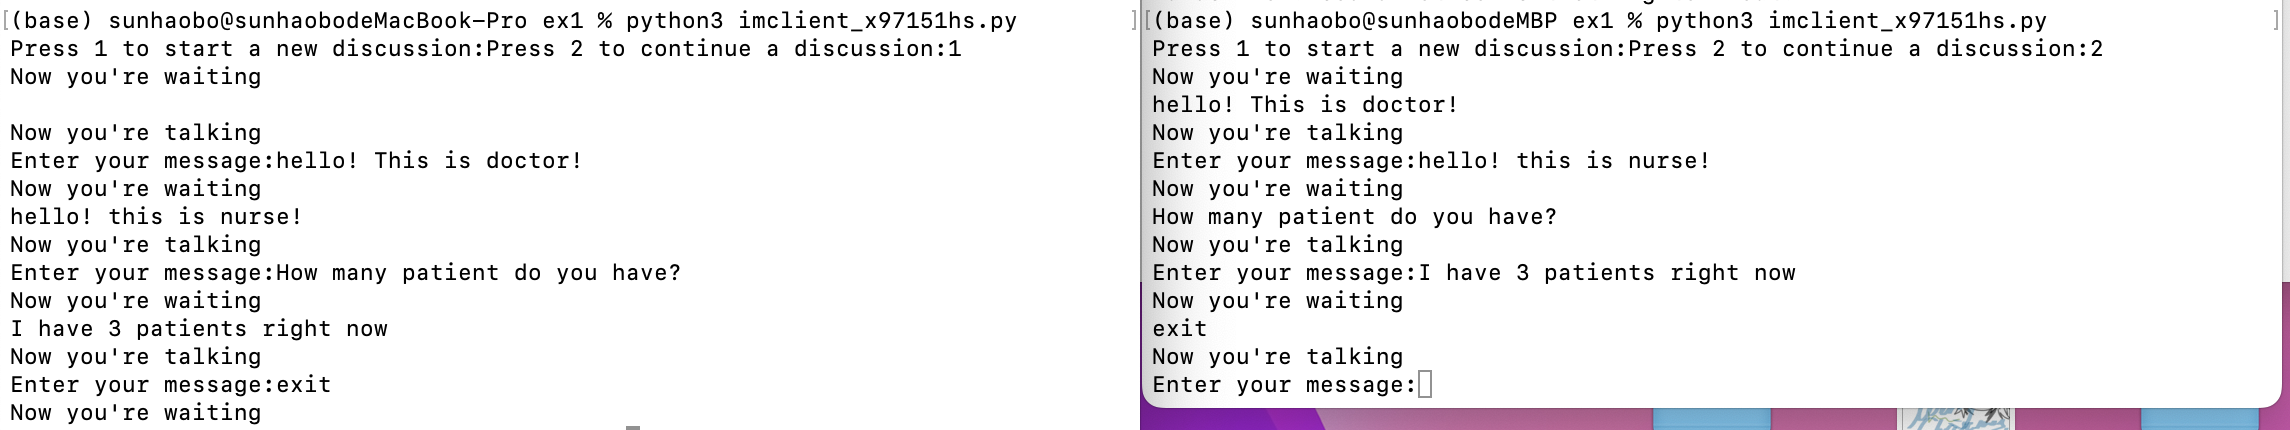
\includegraphics[scale=0.3]{commands.png}
 


\appendix

%% And raw data or code scripts you want to present should be included as appendices.

\end{document}


